%% NYU PhD thesis format. Created by Jos� Koiller 2007--2008.

%%
%% PLEASE SEE THE OFFICIAL FORMATTING GUIDE:
%% http://gsas.nyu.edu/docs/IO/4474/formattingguide.pdf
%% 
%% Style obtained from:
%% http://www.math.nyu.edu/student_resources/misc.php
%%
%% Submission Guidelines:
%% http://gsas.nyu.edu/page/grad.life.dissertation.html
%%

%% Use the first of the following lines during production to
%% easily spot "overfull boxes" in the output. Use the second
%% line for the final version.
%\documentclass[12pt,draft,letterpaper]{report}
\documentclass[12pt,letterpaper]{report}

%% Replace the title, name, advisor name, graduation date and dedication below with
%% your own. Graduation months must be January, May or September.
\newcommand{\thesistitle}{Measurements of Top Quark and Top Quark Like processes at the LHC}
\newcommand{\thesisauthor}{George Herbert Lewis III}
\newcommand{\thesisadvisor}{Professor Kyle Cranmer}
\newcommand{\graddate}{Year of the Depends Adult Undergarment}
%% If you do not want a dedication, scroll down and comment out
%% the appropriate lines in this file.
\newcommand{\thesisdedication}{Dedicated to the memory of Kurt Vonnegut and David Foster Wallace.}


\usepackage{common/atlasphysics}
\def\met{\ensuremath{\not\!\!{E_{T}}}}
\newcommand{\metvec}{{\not\!\! \vec{E}_T}}
\def \Ht {{\rm H}_{\rm T}}
\def\lum{{\ensuremath{\cal L}}}
\def\lumten#1{\ensuremath{10^{#1}\,\mathrm{cm}^{-2}\mathrm{s}^{-1}}}
\def \sp{ \hspace{ 5 pt } }


%% The following makes chapters and sections, but not subsections,
%% appear in the TOC (table of contents). Increase to 2 or 3 to
%% make subsections or subsubsections appear, respectively. It seems
%% to be usual to use the "1" setting, however.
\setcounter{tocdepth}{1}

%% Sectional units up to subsubsections are numbered. To number
%% subsections, but not subsubsections, decrease this counter to 2.
\setcounter{secnumdepth}{3}

%% Page layout (customized to letter paper and NYU requirements):
\setlength{\oddsidemargin}{.6in}
\setlength{\textwidth}{5.8in}
\setlength{\topmargin}{.1in}
\setlength{\headheight}{0in}
\setlength{\headsep}{0in}
\setlength{\textheight}{8.3in}
\setlength{\footskip}{.5in}


%% Use the following commands, if desired, during production.
%% Comment them out for final version.
%\usepackage{layout} % defines the \layout command, see below
%\setlength{\hoffset}{-.75in} % creates a large right margin for notes and \showlabels

%% Controls spacing between lines (\doublespacing, \onehalfspacing, etc.):
\usepackage{setspace}

%% Use the line below for official NYU version, which requires
%% double line spacing. For all other uses, this is unnecessary,
%% so the line can be commented out.
\doublespacing % requires package setspace, invoked above

%% Each of the following lines defines the \com command, which produces
%% a comment (notes for yourself, for instance) in the output file.
%% Example:    \com{this will appear as a comment in the output}
%% Choose (uncomment) only one of the three forms:
%\newcommand{\com}[1]{[/// {#1} ///]}       % between [/// and ///].
\newcommand{\com}[1]{\marginpar{\tiny #1}} % as (tiny) margin notes
%\newcommand{\com}[1]{}                     % suppress all comments.

%% This inputs your auxiliary file with \usepackage's and \newcommand's:
%% It is assumed that that file is called "definitions.tex".
%%
%% Place here your \usepackage's. Some recommended packages are already included.
%%

% Graphics:
\usepackage[final]{graphicx}
%\usepackage{graphicx} % use this line instead of the above to suppress graphics in draft copies
%\usepackage{graphpap} % \defines the \graphpaper command

% Indent first line of each section:
\usepackage{indentfirst}

% Good AMS stuff:
\usepackage{amsthm} % facilities for theorem-like environments
\usepackage[tbtags]{amsmath} % a lot of good stuff!

% Fonts and symbols:
\usepackage{amsfonts}
\usepackage{amssymb}

% Formatting tools:
%\usepackage{relsize} % relative font size selection, provides commands \textsmalle, \textlarger
%\usepackage{xspace} % gentle spacing in macros, such as \newcommand{\acims}{\textsc{acim}s\xspace}

% Page formatting utility:
%\usepackage{geometry}

%%
%% Place here your \newcommand's and \renewcommand's. Some examples already included.
%%
\renewcommand{\le}{\leqslant}
\renewcommand{\ge}{\geqslant}
\renewcommand{\emptyset}{\ensuremath{\varnothing}}
\newcommand{\ds}{\displaystyle}
\newcommand{\R}{\ensuremath{\mathbb{R}}}
\newcommand{\Q}{\ensuremath{\mathbb{Q}}}
\newcommand{\Z}{\ensuremath{\mathbb{Z}}}
\newcommand{\N}{\ensuremath{\mathbb{N}}}
\newcommand{\T}{\ensuremath{\mathbb{T}}}
\newcommand{\eps}{\varepsilon}
\newcommand{\closure}[1]{\ensuremath{\overline{#1}}}
%\newcommand{\acim}{\textsc{acim}\xspace}
%\newcommand{\acims}{\textsc{acim}s\xspace}

%%
%% Place here your \newtheorem's:
%%

%% Some examples commented out below. Create your own or use these...
%%%%%%%%%\swapnumbers % this makes the numbers appear before the statement name.
%\theoremstyle{plain}
%\newtheorem{thm}{Theorem}[chapter]
%\newtheorem{prop}[thm]{Proposition}
%\newtheorem{lemma}[thm]{Lemma}
%\newtheorem{cor}[thm]{Corollary}

%\theoremstyle{definition}
%\newtheorem{define}{Definition}[chapter]

%\theoremstyle{remark}
%\newtheorem*{rmk*}{Remark}
%\newtheorem*{rmks*}{Remarks}

%% This defines the "proo" environment, which is the same as proof, but
%% with "Proof:" instead of "Proof.". I prefer the former.
%\newenvironment{proo}{\begin{proof}[Proof:]}{\end{proof}}


%% Cross-referencing utilities. Use one or the other--whichever you prefer--
%% but comment out both lines for final version.
%\usepackage{showlabels}
%\usepackage{showkeys}

%\usepackage[pdftex]{graphicx}
\usepackage{graphicx}
\usepackage{subfigure}
%\usepackage{atlasphysics}
\usepackage{amsfonts}
%\usepackage{hyperref}
\usepackage[bookmarks]{hyperref}

\begin{document}
%% Produces a test "layout" page, for "debugging" purposes only.
%% Comment out for final version.
%\layout % requires package layout (see above, on this same file)

%%%%%% Title page %%%%%%%%%%%
%% Sets page numbering to "roman style" i, ii, iii, iv, etc:
\pagenumbering{roman}
%
%% No numbering in the title page:
\thispagestyle{empty}
%
\begin{center}
  {\large\textbf{\thesistitle}}
  \vspace{.7in}
  by
  \vspace{.7in}

  \thesisauthor
  \vfill

\begin{doublespace}
  A dissertation submitted in partial fulfillment\\
  of the requirements for the degree of\\
  Doctor of Philosophy\\
  Department of Physics\\
  New York University\\
  \graddate
\end{doublespace}
\end{center}
\vfill

\noindent\makebox[\textwidth]{\hfill\makebox[2.5in]{\hrulefill}}\\
\makebox[\textwidth]{\hfill\makebox[2.5in]{\hfill\thesisadvisor\hfill}}
\newpage
%%%%%%%%%%%%% Blank page %%%%%%%%%%%%%%%%%%
\thispagestyle{empty}
\vspace*{0in}
\newpage

%%%%%%%%%%%%%% Dedication %%%%%%%%%%%%%%%%%
%% Comment out the following lines if you do not want to dedicate
%% this to anyone...
\vspace*{\fill}
\begin{center}
  \thesisdedication\addcontentsline{toc}{section}{Dedication}
\end{center}
\vfill
\newpage
%%%%%%%%%%%%%% Acknowledgements %%%%%%%%%%%%
%% Comment out the following lines if you do not want to acknowledge
%% anyone's help...
\section*{Acknowledgements}\addcontentsline{toc}{section}{Acknowledgements}
%% Write your acknowledgements in this file. If you do not want to acknowledge anyone,
%% you can delete this file and comment out the corresponding part in the "thesis.tex"
%% file.
%

This thesis would not have been possible without the help of many people.
I would like to primarily acknowledge the excellent mentoring of Kyle Cranmer, who has served as my thesis adviser for my graduate school career.
In addition, I would like to thank Allen Mincer and Peter Nemethy for their guidance, advice, and help throughout my time at New York University.
I am indebted to Akira Shibata for teaching me particle physics, computer programming, and for being an excellent example of a productive and successful scientist.
Much of the analysis done toward my degree (and throughout the ATLAS experiment) depended on his contributions to software and measurement techniques.
I would also like to thank Attila Krasznahorkay for the incredible amount of help, both technical and conceptual, that he has provided me over the past few years.
Aside from being an excellent mentor, he has developed and maintained much of the software used to process and analyze the incredible amount of data
produced by the ATLAS detector that made this thesis possible.
I would also like acknowledge Jonathan Zrake for always being available for a discussion, either long or short.
And I would also like to thank Dan Foreman-Mackey for helping to open up the world of computer science to me.
Finally, I would like to thank my parents and the rest of my extended family for their continual support.

%% Write your introduction here.
%
This thesis is about the Riemann Hypothesis. We provide an
affirmative answer to the question ``If $z$ is a zero of the
zeta function and $0\le \Re(z)\le1$, then is $\Re(z)$
necessarily equal to $1/2$?''

In chapter~\ref{chap:one} we do this and that.

In the latter chapters we\ldots


\newpage
%%%% Abstract %%%%%%%%%%%%%%%%%%
\section*{Abstract}\addcontentsline{toc}{section}{Abstract}
%% Write your abstract here.
%
The Riemann Hypothesis has been among the most important open
problems in mathematics for the past 150~years. In this thesis
I solve it, providing a positive result.

\newpage
%%%% Table of Contents %%%%%%%%%%%%
\tableofcontents

%%%%% List of Figures %%%%%%%%%%%%%
%% Comment out the following two lines if your thesis does not
%% contain any figures. The list of figures contains only
%% those figures included withing the "figure" environment.
\listoffigures\addcontentsline{toc}{section}{List of Figures}
\newpage

%%%%% List of Tables %%%%%%%%%%%%%
%% Comment out the following two lines if your thesis does not
%% contain any tables. The list of tables contains only
%% those tables included withing the "table" environment.
\listoftables\addcontentsline{toc}{section}{List of Tables}
\newpage

%%%%% Body of thesis starts %%%%%%%%%%%%
\pagenumbering{arabic} % switches page numbering to arabic: 1, 2, 3, etc.

%% Introduction. If your thesis has no introduction, or chapter 1 is
%% meant to be the introduction, then comment out the lines below.
\section*{Introduction}\addcontentsline{toc}{section}{Introduction}


%% Write your introduction here.
%

%Before it was discovered in 1995 by the Tevatron, the existance of the top quark was nearly assured.

% To add:
% - The Standard Model
% - What isn't in the standard model
% - Results that need to be explained


The top quark is the most massive fundamental particle in the Standard Model of particle physics.
Discovered in 1995 at the Tevatron by both the CDF and D0 experiments, it was the final piece in the quark model described by the Standard Model theory of fundamental particle physics.
Long before it was confirmed experimentally, the existance of the top quark was assured as it was required for the consistency of the Standard Model.
Its presence is necessary to prevent anomalies and high energy divergences, to explain the measured properties of the couplings of the $b$-quark to the $Z$ boson, and to explain a number of precision electroweak measurements.

%The top quark is the most massive fundamental particle in the Standard Model of particle physics, including the recently discovered Higgs boson.
At 173 GeV \cite{PARTICLE_DATA_GROUP}, it weights about as much as a gold nucleaus and is significantly more massive than the next heaviest quark.
The reason is it so massive (even more massive than the recently discovered Higgs boson) remains unknown.
Its status as the most massive known fundamental particle has lead to speculation as to whether it plays a special role in electroweak symmetry breaking, or perhaps that its large mass is intimately tied to the solution of the hierarcy problem.
%http://arxiv.org/pdf/1206.4484v1.pdf

The top quark also plays an important role in many scenerios proposing new physical models.
Many proposed massive particles decay preferentially into top quarks or are the result of top quark decays.
Moreover, the production and subsequent decay of the top quark leads to an experimental signature that can be extremely useful in searches for new physics.
And many new physical models can be indirectly probed using the precision measurement of the properties of the top quark.
% http://www.osti.gov/accomplishments/documents/fullText/ACC0202.pdf

Because of its mass, the top quark decays almost immediately.
This means that it is the only quark whose properties can be directly measured, as it decays before it can before it can participate in low energy QCD processes that make the direct measurement of lighter quarks difficult.
% http://cms.web.cern.ch/news/precision-measurements-using-top-quarks-cms

The LHC is often described to as a ``top factory,'' referring to the incredible rate of top-quark production due to its high energy and luminosity beam.
The abundence of top quark events produced by the LHC allow for high precision measurements of the properties of the top quark.
The precise measurement of it's properties not only serves as a crucial test of the capibalities of the Large Hadron Collider and the ATLAS detector, but serves as an excellent way to search for Beyond the Standard Model physics.
Moreover, these measurements are an excellent application of state-of-the-art statistical techniques which have been developed to enable deep and precise measurements by the experiments at the LHC.
%Precise measurements of the Top Quark's properties require experimental and statstical techniques.

This thesis will describe two types of measurements that were used to study the Standard Model and to search for physical models proposed to explain beyond the Standard Model physics.
The first measurement is a sophisticated and precise determination of the top quark pair production cross-section at a center of mass energy of $\sqrt{s} = 7$ TeV.
The second is a search for exotic physical particles and signatures that lead to final states containing or resembling two or more top quarks.

%The top-quark pair-production cross-section has been previously measured at the Tevatron with the CDF and D0 experiments.
%The CDF result, using single-lepton decay channels, obtained a cross-section measurement at 1.8 TeV of $\sigma_{t\bar{t}} = 6.5^{+1.7}_{-1.4}$ pb. %http://arxiv.org/abs/hep-ex/0101036
%Similarly, D0, using nine decay channels, measured a cross-section of $5.69 \pm 1.21$ (stat) $\pm$ 1.04 (sys) pb, assuming a top quark mass of 172.1 GeV.

%The precise measurement of it's properties not only serves as a crucial test of the capibalities of the Large Hadron Collider and the ATLAS experiment, but serves as an excellent way to search for Beyond the Standard Model physics.

%Precise measurements of the Top Quark's properties require experimental and statstical techniques.

\clearpage
\newpage

%
%
%

\section{ATLAS}
ATLAS is a multi-purpose particle detector designed for particle discovery.
In order to fulfull this broad role, ATLAS must excel in several ways:

\begin{itemize}
  \item It must be sensitive to a wide spectrum of particle that can be produced by particle colissions, including Leptons (Electrons and Muons), Hadrons (Pions, Kaons, and the many other bound states of quarks that typically come in the form of Jets), and Photons.
  \item It must be able to identify precisely the kinematic properties of these particles, which includes measuring their energies and directions with a high resolution.
  \item It must maintain its resolution over a large range of energies, roughly from 1 GeV up to and including the TeV scale.
  \item It must make these measurements at an extremely high rate, millions of times a second, and over the entire lifetime of the experiment, which could end up being decades
  \item It must be able to record, save, and successfully distribute its collected data to experimentalists and analyzers around the world.
\end{itemize}

These requirements are entirely non-trivial, and fulfilling them required decades of design, construction, engieneering, and maintenence.  
The original design for ATLAS
In order to be successful, ATLAS 
to use a wide spectrum of detector designed to discover particles and to precisely measure their proproperties.


Typical descriptions of the ATLAS detector list its various components and describe their properties.
But perhaps it is more useful to instead approach the detector from the perspective of the different particles that it is designed to detecct, and to use that as a springboard to go into machine's enieneering details.

\subsection{Layout and Geometry}
Cylander, eta, phi size, underground, lhc, geneva, Mount Blanc, etc


\subsection{Overview}
ATLAS is a multi-component detector consisting of many individual subsystems, each of which measures a certain number of kinematic properties of particles created or scattered by the LHC.
Only when combining the measurements of these sub-systems do complete pictures of particles and entire begin to emerge.
The subcomponents of ATLAS are layered around the central location of the primary interaction.
The inner-most layer of ATLAS is the ``inner detector'', which consists of silicon strips and pixils and is designed to track the 3-d trajectories of charged particles passing through it.
The inner detector extends for 1.15 m and is surronded by a solonodial magent which provides a 2T field within the inner detector.
This field causes charged particles to bend and allows the inner detector to measure the momenta of charged particles by fitting their trajectories.
Surronding the inner detector is the electromagnetic calorimeter, which consists of alternating layers of lead absorbers and active electronics that are baithed in liquid argon.
The liquid argon must of course remain cooled, and so the electromagnetic calorimeter is located within a cryostat that maintains a temperature of [XX].
To reduce the amount of upstream material present before the calorimeter systems, the solonodial magent for the inner detector is located within the EM calorimeter's cryostat.
A dedicated presampler is located directly behind the cryostat's wall to correct for any energy lost within inactive material in front of the EM calorimeter.
Behind the outside of the cyrostat and past the EM calorimeter is the hadronic calorimeter, which consists of alternating layers of iron and scintillating tile.
Finally, the outer-most layer of ATLAS is the muon spectrometer, which consists of many subsystems designed to detect the trajectories of muons at high rates and with good resolution. 
A 8T magnetic field is induced across the entire muon system and is produced by large superconducting toroid magnets.

\subsection{Inner Detector}
The inner detector is first part of the ATLAS detector encountered by particles emerging from the interaction point.
The inner detector (ID) consists of three subsystems which are designed to track the trajectories of charged particles as a collection of discrete points where they hit active parts of the detector.

The first layer of the ID is the pixel detector, which itself consists of three barrel layers of pixel modules at radaii of 4 cm, 10 cm, and 13 cm (on average) as well as five disks on each side of the deterctor to cover the forward region in pseudorapidity.
Each region contains a collection of pixel modules (which are identical across the barrel and disk regions) which are 62.4 mm long and 21.4 mm wide.
The individual modules contain 61,440 pixel elements, and there are 1500 such modules in the barrel and 700 in the disks. %read out by 16 chips, each serving an array of 24 by 160 pixels 
In total, there are about 140 million detector elements. % each 50 μm in the Rφ direction and 300 μm in z,
The pixel detectors are designed to measure the impact parameters of short-lived particles lead to non-neglegable displaced vertices, such as $\tau$s and b-quarks.
% Pixel Image: http://www.atlas.ch/pixel-detector.html
% Paper and individual pixel image: http://arxiv.org/pdf/physics/0412138.pdf

Moving outward through the inner detector, the next layer encountered is the Semiconductor tracker (SCT).
Since it exists at a larger radius, the SCT must cover a larger area (about 61 $m^2)$ with active material.
The detector contains 6.2 million readout channels that are spread across four complete barrels at radii of 30.0, 37.3, 44.7 and 52.0 cm, and three rings of end-cap detectors on either side.
Each subdetector consists of a collection of 6.36$\times$6.40 $cm^2$ silicon strips (each with 768 readout strips) arranged in an overlapping pattern with each strip aligned at a small angle.
The spatial resolution is of the SCT is 16 $\mu$m in $R-\phi$ and 580 $\mu$m in z, which can distinguish tracks that are separated by as little as 200 $\mu$m.

The final component of ATLAS' inner detector is the Transition Radiation Tracker (TRT).

\subsection{Electromagnetic Calorimeter}
The subcomponents that make up ATLAS's electromagnetic calorimeter are each designed to measure the energy of electrons and photons by inducing and absorbing an elecromagnetic shower.
Heavier charged particles, such as muons and pions, will interact with electromagnetic calorimeters, but their interaction lengths are longer than those of electrons and photons, which makes their showers more elongated.
As a result they do not deposit a majority of their energy within the range of ATLAS' EM calrimeters.
ATLAS' Electromagnetic calorimeter is divided into three subsections consisting of the barrel calorimeter, which covers a pseudorapidity range of $|\eta| < 1.475$ and the two end-cap calorimeters, which covers $1.375 < |\eta| < 2.5$.
However, as opposed to the hadronic calorimeter, each subcomponent shares a common design.
The calorimeter consists of layers of lead absorbers shaped in a zig-zag, accordian-like pattern and similarly arranged Kapton electrodes placed in the middle of gaps between the lead absorbers.
%The calorimeter consists of alternating layers of Kapton electrodes and lead absorbers that are both shaped in a zig-zag, accordian-like pattern.
The calorimeter's zigs and zags are aligned in the radial direction, which removes the possability of inactive cracks where two plates meet.
The entire calorimeter is bathed in liquid argon, which is maintained at a temperature of about 88 degrees kelvin by the cryostats that encases the electromagnetic calorimeters (for this reason, ATLAS' electromagnetic calorimeters are commonly referred to simply as the ``LAr calorimeter'').
As charged particles fly through the calorimeter, they will ionize the Liquid Argon, and ionized electrons are drawn toward the active electrodes by a high voltage electric field (of about 1 kV/mm) that is maintained throughout the calorimeter. % [http://arxiv.org/pdf/0912.2642v4.pdf]
The current absorbed is preportional to the energy deposited, which is used to reconstruct the energy of the electron hitting the calorimeter.
Each LAr calorimeter is segmented into three or four transverse layers and is divided into cells of varying granularity in  $\Delta \eta \times \Delta \phi$, depending on the location and on the layer.%$ = 0.1 \times 0.1$ for $|\eta| < 2.5$ and up to $\Delta \eta \times \Delta \phi = 0.4 \times 0.4$. for $3.1 < |\eta| < 4.9$.
In all, the LAr calorimeter has 182,468 readout cells.
Of particular importance is the first layer of very LAr barrel calorimeter, which is finely segmented ``strips'' of  $\Delta \eta \times \Delta \phi = (0.0031 \times 0.098)$. 
This this $\eta$ segmentation allows for the resolution of the EM shower shape differences between photons and $\pi_{0}$s which decay into narrowly separated photon pairs, 
In the barrel, the three layers of LAr calorimeters have thicknesses of 4.3, 16, and 2 radiation lengths, respectively.
In addition, the barrel contains a presampler layer, which consists of LAr electrods, but no lead absorber, that is used to correct for energy lost in the inner detector, the solenoid magnet, and in the cryostat walls (the end caps have less material upstream from the EM calorimeters and therefore don't require a presampler). % [http://www.hep.lu.se/atlas/thesis/egede/thesis-node43.html]

% Helpful Talk: [http://www.physics.utoronto.ca/~krieger/talks/Krieger_NSS05_Talk.pdf]
% Commissioning ATLAS paper: [http://arxiv.org/pdf/0912.2642v4.pdf]
% LAR Temperature: [http://cdsweb.cern.ch/record/686091]


\subsection{Hadronic Calorimeter}
The Large Hadron Collider is thus named because it collides a specific hadronic bound state of quarks known as the proton.
The majority of interactions between these particles are mediated by the strong force (QCD), and the vast majority of final state particles are cone-like sprays of hadronic particles known as Jets.
It is therefore crucial that a detector working with a hadron collider be excellent at identifying and measuring hadronic particles.

% General Hadronic Calo layout
The primary means of studying a jet is through calrimetry, where the energy of a jet is determined by stopping its hadronic shower using a dense material and measuring the energy it deposits in an active material.
The direction of the jet is determined by the  $\eta$, $\phi$ location of where the jet hits the detector.
The ATLAS hadronic calorimeter is designed to contain as much of a hadronic shower within the calorimeter itself and to accurately determine its energy using the calorimeter's active components.
It is divided into three subsystems that cover overlapping ranges in pseudorapidity.
The largest and most important is the ``tile'' hadronic calorimeter (which itself is divided into the ``barrel'' and two ``extended barrel'' tile calorimeters), which covers the rapidity region of $|\eta| < 1.7$. [tdr]  
The ``hadronic end cap'' (HEC) extends the calorimeter's range up to $|\eta| < 3.2$, and the ``forward calorimeter'' (FCAL) covers the pseudorapidity range of $3.1 < |\eta| < 4.9$.  
%Each of these subsystems have similar goals but vary in their design.

% [pdg review: http://pdg.lbl.gov/2011/reviews/rpp2011-rev-passage-particles-matter.pdf]

% [http://rd11.web.cern.ch/RD11/rkb/PH14pp/node80.html]

% The Tile
The hadronic tile calorimeter, which covers [XX] starradians, detects jets that emerge low pseudorapidity, including those that are close to perpendicular to the beam pipe.
It is a cylindric shell ranging from an inner radius 2.28 meters and outer radius 4.25 meters.
The tile is made of three subsystems, one central ``barrel'' calorimeter which covers $|\eta| < 1.0$ and two ``extended barrel'' calorimeters, which cover $0.8 < |\eta| < 1.7$ on either side.
The tile calorimeters consist of alternating layers of 14 mm iron plates, which is used for inducing the hadronic shower and stopping the jet, and 3mm active scintillating-tile, which is used to measure the energy deposited into the calorimeter by the jet.
%Iron is used because the hadronic particles that make up jets interact strongly with nucleii, and therefore a material with a high nuclear density is desirable.
The scintillating tile is attached to a series of photomultiplier tubes (PMTs) that amplify the tile's electrical readout.
Key to the successful performance of the tile calorimeter is providing enough average interaction lengths for the hadronic shower to be contained.
The hadronic thickness at the end of the tile calorimeter (at $\eta=0$) is 9.2 $\lambda$, which is enough to ensure good jet resolution and to minimize jet ``punch through'' into the muon system.



\subsection{Muon Spectrometer}

\subsection{Measuring Particles with ATLAS}

\subsection{Jets}
Jets are produced when particles with color charge, quarks and gluons, are in the outgoing states of a hard interaction.
As these particles propogate through space, they will tend to decay into or radiate other color-charged particles, leading to a phenomenon known as the evolution of a ``parton shower.''
This shower grows rapidly because QCD, which is an asymptotically free field theory, has a small coupling constant at high energies.  
As the shower progresses and the average energy of the constituent particles decreases, the QCD coupling constant will grow stronger, and this will cause the quarks and gluons to bind together into stable particles in a process known as ``hadronization.''
The collection of these hadrons, which move in a wide, cone-like shape, is known as a jet.
%The average distance for the parton-shower, hadronization evolution process is small compared to the radius of ATLAS, adn so jets are fully formed as they begin to interact with the detector

A jet originating from the beam spot and and moving through ATLAS will first interact with the inner detector.  Since many of the constituent particles of a jet are charged hadrons ($\pi^{+}$, $K^{+}$, etc), they will leave tracks in the ID.
Jet algorithms can use these tracks when attempting to identify a jet, and there are algorithms that exclusively rely on this collection of tracks to build a set of identified jets (

%[ Track Jets, 2009: https://atlas.web.cern.ch/Atlas/GROUPS/PHYSICS/CONFNOTES/ATLAS-CONF-2010-002 ].

However, the most common way to reconstruct jets is using the calrimetry.
Jets will deposit a small fraction of their energy in the Electromagnetic Calorimeter, but the majority of the shower's energy is measued by the hadronic calorimeter.
There are many algorithms used to reconstruct jets using information from the hadronic calorimeter, but most of them consist of clustering algorithms which group together cells of energy deposits.
The main differences between techniques involve how these energy deposits are calibrated (if at all) and how the cells are clustered (based on fixed geometries, such as cones, or based on iterative algorithms using a distance function to merge cell deposits).
A small number of jets managed to escape the hadronic calorimeter and enter the muon chambers, where they can be misidentified as mouns.
In addition, jets with ``heavy flavor'' may contain decays that result in real muons (but not muons that originated from a hard collission in the beam spot), so care must be taken to separate muons originating as jets from muons originating from the hard process.

% How jets work, and how they shower

%% The first step in measuring a jet's energy is stopping it.  
%% The hadronic partilces that make up a jet are made up of quarks and gluons, which are charged under the strong force (QCD).
%% They therefore interact with the nucleii of materials that they pass through.
%% The primary mechanism for energy loss of high energy hadrons traveling through a solid material is via inelastic nuclear interactions.
%% As these interactions cause the original hadron to lose energy, they will also cause nuclear excitations and subsequent nuclear decays in the material.
%% This in turn leads to the emission of additional hadronic particles, which themselves will interact with the material.
%% The net effect is the formation of what is known as a hadronic shower.
%% When the energy of the daughter particles in the shower becomes too small for nuclear excitation, the shower ceases to evolve, and the remaining energy of hadrons is lost to ionization and electromagnetic interactions.
%% While the majority of energy is lost via nuclear interactions, a non-neglegable fraction of a jet's energy interacts electromagnetically .
%% This fraction 


\subsection{Electrons}
Electrons and positrons are electromagnetically charge and wil therefore interact with the innner detector, and in addition their trajectories will be curved as the particles are beant by the magnetic field.
As they pass through the inner detector, electrons will deposit hits in the pixles, silicon, and straw tubes, and the collection of these hits can be extrapolated together to reconstruct the electron's track.
This track is of crucial importance for identifying electrons.
The track carries information both about the direction of the electron, but also about its momentum, and the presence of a track is necessary to distinuish electrons from photons, which lead essentially identical electromagnetic showers in the EM calorimeter.
When electrons enter the EM calorimeter, they will begin to decellerate, which will cause the electron to radiate via bremsstralung.
The radiated photons often have enough energy to produce electorn-positron pairs, which themselves will emit bremsstralung radiation.
This creates a cascade of electrons, positrons, and photons that is collectively known as an electromagnetic shower.
The energy of this shower is determined as it is absorbed by the EM calorimeter.
The EM calorimeter tends to provide a better energy resoltion for high pT electrons than the tracks do (beginning when the electron's energy is around 10 GeV).

% [ 2010 performance: http://cdsweb.cern.ch/record/1273197 ]
% [ https://atlas.web.cern.ch/Atlas/GROUPS/PHYSICS/PUBNOTES/ATL-PHYS-PUB-2011-006/ATL-PHYS-PUB-2011-006.pdf ]
% [ Moriond 2012 Resolution info: https://indico.cern.ch/getFile.py/access?contribId=3&resId=1&materialId=slides&confId=163471]
% [ https://twiki.cern.ch/twiki/pub/AtlasProtected/EnergyScaleResolutionRecommendations/summary_rel16.pdf ]

\subsection{Photons}
Photons are identified as electromagnetic showers that aren't matched to an inner detector track.
In addition, photons may decay into an electron-positron pair before entering the EM calorimeter.
If this occurs within or before the inner-detector, the proximity of the electron and positron's tracks can be used to identify the pair as a photon that ``converted'' electromagnetically, and the pair can be reconstructed as a single photon.
%In addition, photons may be identified as electron-positron pairs  from ``conversions,'' which are electron-positron pairs that 


\subsection{Muons}
Muons, with a mass of 106 MeV, weigh about 200 times more than the electron (which weights .512 MeV).
This implies that, for a fixed energy, a muon will have a smaller value of $\beta$ than an electron (or, equivalantly $\gamma$), which results in a smaller amount of radiation being emitted as it passes through matter.
Therefore, a muon's mean radiation length in ATLAS' calorimeters will be much longer than an electron's length, and a significant EM shower will not develop within the detector.
For this reason, most of a muon's energy escapes ATLAS.  

% [ pdg: Muons through matter: http://pdg.lbl.gov/2000/passagerpp.pdf fig 23.1 ]

Since one can not measure its energy through calrimetry, ATLAS instead measures its momentum by estimating its curvature when bent in a magnetic field.
A Muon will create a bent track in the inner detector that can be used to estimate its momentum.
However, the resolution of the inner detector for high pt muons becomes somewhat poor.
To vastly improve on the measurement of the inner detector alone, ATLAS has a large set of detectors that comprise the muon spectrometer.

\clearpage
\newpage

%
%
%

\section{Top Quark Pair-Production Cross-Section Combination}

A precise measurement of the Top Quark Pair-Production Cross-Section is crucial for understanding the performance of the ATLAS detector, for testing predictions of the standard model, to searching for or constraining many new physical models.
In particle physics, a cross-section is a way to describe the rate of a specific interaction or class of interactions independently of beam conditions that are used to produce it.
The value of the top-quark pair-production cross-section in the Standard Model can be predicted using Monte-Carlo simulation techniques \cite{TOP_XSC_THEORY} \cite{TTBAR_HADRON_COLLIDERS} \cite{THRESHOLD_EXPANSION_XSC}.
This value can be determined using ``Next to Leading Order'' techniques (NLO) and is corrected by adding the ``Next to Next to Leading Order'' soft logarithm terms (approximate NNLO).
This value is determined to be $\sigma_{\ttbar} = 165^{11}_{16}$ with an uncertainty below 10\%.
The most accurate experimental determinations of the top quark's cross section previous to the LHC's results were measured by the CDS and the D0 collaborations at the Tevatron \cite{TEVATRON_XSC_LJETS} \cite{TEVATRON_XSC_DILEP}.
These experiments determined the cross-section at a center-of-mass energy of $\sqrt{s} = 7 TeV$ to a precision of 8\% using individual channels and 6.4\% by combining measurements across multiple channels.

The top-quark pair-production cross section has been measured at ATLAS using many channels and analysis technqiues.
The most precise measurements use combination of several individual measurements, which reduces both statistical and systematic uncertainties.
This section presents an ATLAS measurement of the $\ttbar$ cross-section that statistically combined three separate analysies strategies.
The likelihoods for measurements using single-lepton, dilepton, and all-hadronic channels were modeled as functions of the top cross-section, as well as a variety of nuisance parameters.
% This combination was performed by modeling the likelihoods of several individual measuremnets as functions of the top cross-section as well as a variety of nuisance parameters.
These likelihoods were then merged and a simultaneous fit to the measured data across all channels was performed.

The combined measurement of the $\ttbar$ cross-section used a measurement in the lepton+jets channel which was performed using 0.7$\ifb$ of data recorded in 2011 \cite{LEPTON_JETS_NOTE_2011}, a measurement in the dilepton channel which was performed using XX, and a measurement in the all-hadronic channel, which was performed using XX.


\subsection{Top Quark Pair-Production}

The primary means of producing top quarks at the LHC is via gluon fusion and subsequent decay into a pair of top quarks.

\begin{figure}
  \begin{center}

    \subfigure[Production]{
      % TopQuarkPairProductionDiagram: http://kjende.web.cern.ch/kjende/netzwerk/images/Feynman/WplusWminusBBar.png
      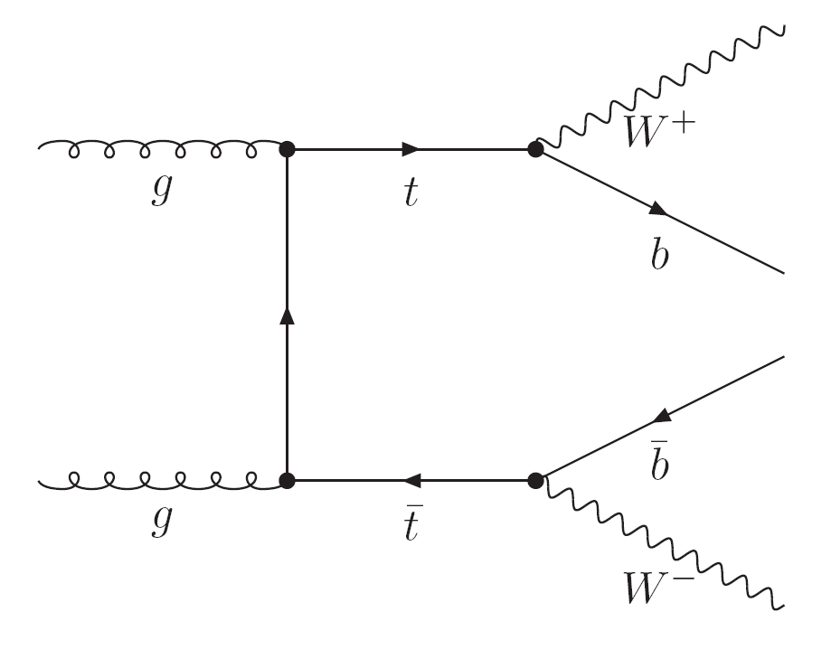
\includegraphics[width=.4\linewidth]{figures/xsection/TopQuarkPairProductionDiagram.png}
    }
    \subfigure[Decay]{
      % TopQuarkBranchingRatios: http://ej.iop.org/images/0034-4885/75/5/056201/Full/rpp347183f06_online.jpg
      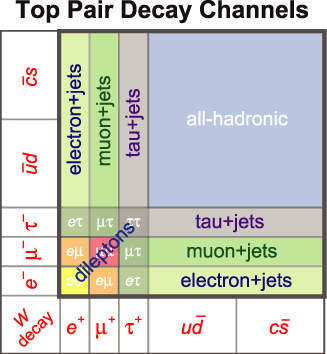
\includegraphics[width=.4\linewidth]{figures/xsection/TopQuarkBranchingRatios.jpg}
    }
  \end{center}
  \caption{ A typical feynman diagram of top quark pair production at the LHC.  Top quarks decay into W-bosons and b-quarks nearly 100\% of the time.  The subsequent decays of the W-Bosons determine the event topology of the \ttbar event.  Diagram showing the branching ratios of Top Quark pairs into leptons and quarks.}
  \label{img:TopQuarkPairProduction}
\end{figure}

W bosons decay either leptonically, in which they produce a lepton and a neutrino, or hadronically, in which they produce a pair of quarks.
W's decay leptonically XX\% of the time, which consists of decaying via $W- \rightarrow e \bar{\nu_{e}}$ 10.75\% of the time, via $W- \rightarrow \mu \bar{\nu_{\mu}}$ 10.57\% of the time, and via $W- \rightarrow \tau \bar{\nu_{\tau}}$ 11.25\% of the time, and decay into quarks the other 67.60\% of the time. % [pdg]
% W-Boson: http://pdg.lbl.gov/2012/listings/rpp2012-list-w-boson.pdf
However, tau leptons are themselves unstable particles that subsequently decay either leptonically (muon 17.41 or electron 17.83), or hadronically 64.76\% of the time, with about 50\% of the tau's today decays into 1 hadron and 15\% into 3 hadrons.
% Tau pdg: http://pdg.web.cern.ch/pdg/2012/listings/rpp2012-list-tau.pdf
In the discussion that follows, we will consider the $W \rightarrow \tau  \rightarrow e$ or $W \rightarrow \tau  \rightarrow \mu$ to be leptonic decays of the top, and we will ignore the intermediate state $\tau$ in terms of our classification.
Hence, a pair of top quarks, which we assume always decay into a pair of W bosons, will decay into two leptons 6.5\% of the time (known as the ``dilepton'' channel), into a single lepton and a pair of quarks 34.4\% of the time (known as the ``single lepton'' channel), and entirely into quarks 45.7\% of the time (known as the ``all hadronic'' channel).
% pdg:
% Citation: J. Beringer et al. (Particle Data Group), PR D86, 010001 (2012) (URL: http://pdg.lbl.gov)



%% \begin{figure}
%%   \begin{center}
%%     % TopQuarkBranchingRatios: http://ej.iop.org/images/0034-4885/75/5/056201/Full/rpp347183f06_online.jpg
%%     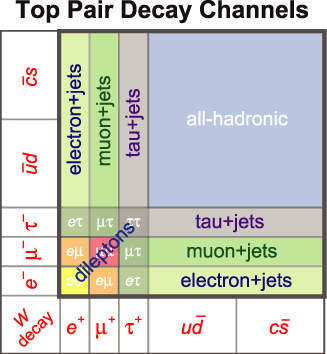
\includegraphics[width=100mm]{figures/xsection/TopQuarkBranchingRatios.jpg}
%%   \end{center}
%%   \caption{}
%%   \label{img:TopQuarkBranchingRatios}
%% \end{figure}

\subsection{Object Reconstruction}

Measurements of $\ttbar$ event require kinematicaly reconstructing and selecting a variety of physical objects, including electrons, muons, jets, b-jets, and $\MET$.

% Selected Electrons
Selected electrons are required to have a calorimeter cluster located in a pseudorapidity range of $0 < |\eta| < 4.47$, excluding the range $1.37 < |\eta| < 1.52$ (this excluded interval, known as the crack region, is a mostly un-insturmented part of the EM calorimeter).
To reject jets that fake electrons, the electron's energy is required to be isolated in the calorimeter.
Specifically, electrons with more than 3.5 GeV of energy in a cone of $\sqrt{(\Delta \eta)^2 + (\Delta \phi)^2}$, excluding the energy of the electron itself, are rejected.
Electrons must pass a variety of cuts related to the shape of its shower and the quality of its corresponding track that are collectively referred to as ``tight'' EM identification cuts.
Finally, Electrons must have a minimum energy of $E_{T} > 20$ GeV, where $E_{T}$ referrs to the transverse energy of the electron's electromagnetic cluster..

%% The selection of l + jets tt ̄ events makes use of reconstructed electrons, muons and jets, and the transverse momentum imbalance referred to as missing transverse energy Emiss.
%% T Electron candidates are reconstructed from the energy depositions in the electromagnetic calorimeter
%% and are required to have a well-measured track associated with the electromagnetic cluster. The latter is required to have |ηcluster| < 2.47 excluding 1.37 < |ηcluster| < 1.52 corresponding to the transition region between barrel and endcap calorimeters. To ensure that electrons are isolated from the jet activity, as expected for prompt electrons from W boson decay, the energy in a cone of ∆R ≡ 􏰮∆η2 + ∆φ2 = 0.2, centered around the electron, excluding the energy associated with the electron itself, is required to be < 3.5 GeV. This defines the tight electron candidates used for the final analysis. Loose electron candidates employed for the estimation of the QCD multijet background, as described in Section 4, have to fulfill less stringent requirements and the isolation cut is increased to < 6 GeV energy deposition in ∆R = 0.2.

% Selected Muons
Selected Muons must be ``combined'', meaning they must use tracks from both the muon spectrometer and the inner detector.
Only muons within $|\eta| < 2.5$ are considered, and muons within $\Delta R <= 0.4$ of a selected jet are rejected.
Two isolation requirements are imposed on selected muons.  
They must be isolated in the calorimeter, meaning the energy deposited in the calorimeter within $\Delta R = 0.3$ must be $<$ 4 GeV, and their tracks must be isolated, meaning the sum of the transverse momenta of tracks in a code of $\Delta R = 0.3$ surronding the muon's track must be $<$ 4 GeV.

%% Muon candidates are reconstructed by searching for track segments in the different layers of the muon spectrometer. These segments are then combined starting from the outermost layer, and matched with the inner detector tracks. The final parameters of muon candidates are obtained from the combined fit using information from both detector systems. Only muons within |η| < 2.5 are included in this measurement. Like electrons, muons are required to be isolated, i.e. (i) be separated from the closest jet by ∆R(μ, jet) > 0.4; (ii) have calorimeter isolation < 4 GeV and (iii) have track isolation < 4 GeV. Track isolation is defined as the sum of track transverse momenta in a cone ∆R ≡ 􏰮∆η2 + ∆φ2 = 0.3, excluding the pT of the muon track, while calorimeter isolation is defined as energy deposition in the calorimeter within a cone of ∆R = 0.3, excluding the energy deposition directly along the muon track. Muons passing all requirements are used in the analysis sample selection and are referred to as tight, while muons with a looser isolation are used for the QCD multijet background estimate described in Section 4. In this case, all requirements except the cuts on calorimeter and track isolation have to be fulfilled and the muons are referred to as loose.


% Selected Jets
In this analysis, Jets are constructed using the anti-kt algorithm with a distance parameter of $R=0.4$.
These jets are built out of ``topoligical clusters'', which themselves are collections of neighboring cells that each have an energy above some threshold, where the energy has been calibrated to the scale of electromagnetic showers (known as ``Electromagnetic Scale'').
Once the jets are built, their energies are then recalibrated to the scale of hadronic particles (known as the ``Hadronic scale'') \cite{JES_SCALE_2010}.
Since jets are built out of calorimeter deposits, essentially all electrons will also be reconstructed as jets.
Therefore, these objects must be removed from the collection of selected jets by-hand.
In this analysis, any jet that overlaps with a selected electron within $\Delta R < 0.2$ is removed.

%% Jets are reconstructed using the anti-kt algorithm with distance parameter R = 0.4 [9] which sets the relative distance at which jets are resolved from each other. As input, the algorithm uses topological clusters that group together neighboring calorimeter cells with energy deposits above certain thresholds. Their energy accounts correctly for the energy deposited in the calorimeter by electromagnetic showers. Additional correction factors dependent on jet η and pT are applied to the reconstructed jets to correct their energy to the hadronic scale. The jet energy scale (JES) is established using corrections derived from collision and test beam data and calibration constants obtained from MC simulation [10]. Since reconstructed electrons might also be reconstructed as jets in the calorimeter, any jet overlapping with a %% 2 %% tight electron within a cone of ∆R < 0.2 is removed from the list of jets. 

%% MET
Finally, once all objects have been selected, the $\MET$ is defined as the vector sum of the calorimeter energy deposits of selected objects or the combined energy for muons (including additional corrections for energy deposited in the calorimeter).
The energy associated with each object is calibrated to the scale of that object, and all remaining energy deposits are added to the $\MET$ vector, but at electromagnetic scale.


%% The analysis reconstructs the missing transverse energy from the vector sum of energy depositions
%% in the calorimeter in the transverse plane associated to the objects used in the analysis. The same recon-
%% struction and identification algorithms as for the analysis objects are used to identify electrons and jets.
%% The corresponding topological clusters in the calorimeters are then included in the calculation of Emiss at T
%% the energy scale of the associated object. The muon momenta are calculated using the information from both the inner detector and the muon spectrometer system and corrected for additional energy deposi- tion in the calorimeter. Remaining energy depositions not associated to any object are included at the electromagnetic energy scale.


%% END


\subsection{Lepton+Jets}
The lepton$+$jets channel is the most statistically powerful decay of the $\ttbar$ system for measuring the pair-production cross-section.
The leptonic decay of one of the top results in an event topologiy that allows for strong background discrimination, while the hadronic decay of the other top maintains a high branching ratio for this channel.
The distinguishing features of the lepton$+$jets channel is the presence of a high-pt lepton from the leptonic decay of a W boson,$\MET$ from a neutrino, two b-jets from the decay $t \rightarrow W+b$, and two additional jets from the hadronic decay of a W boson.



\subsubsection{Backgrounds}
A selection of events based on the above criteria will be contaminated with several sources of backgrounds, including

\begin{itemize}
\item QCD Multijet events where a lepton is faked via a background mechanism
\item $W+Jets$ events where the W decays leptonically (leading to $\MET$) which includes real or fake b-jets
\item $Z+Jets$ events where one of the two leptons isn't identified and which includes real or fake b-jets
\item Diboson Events (WW, WZ, or ZZ events), that include some combination of leptonic decays of vector bosons, additional jets, and real or faked b-jets
\item Single Top events
\end{itemize}

% Add figures

\begin{figure}
  \begin{center}
    \subfigure[$Z+Jets$]{
      %ZJetsDiagram.png : http://inspirehep.net/record/871058/files/qg_qZ.png
      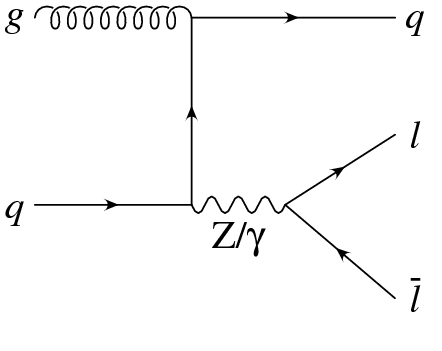
\includegraphics[width=.4\linewidth]{figures/xsection/ZJetsDiagram.png}
    }
    \subfigure[$W+Jets$]{
      % 
      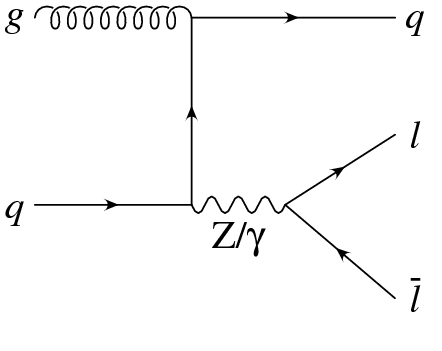
\includegraphics[width=.4\linewidth]{figures/xsection/ZJetsDiagram.png}
    } \\
    \subfigure[$QCD$]{
      %ZJetsDiagram.png : http://inspirehep.net/record/871058/files/qg_qZ.png
      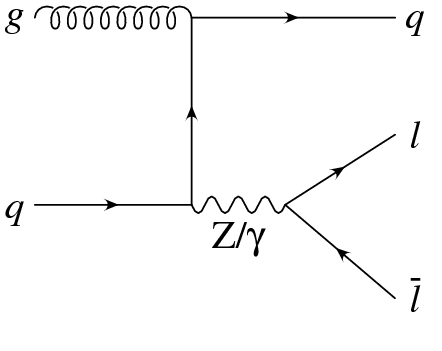
\includegraphics[width=.4\linewidth]{figures/xsection/ZJetsDiagram.png}
    }
    \subfigure[$Single Top$]{
      % 
      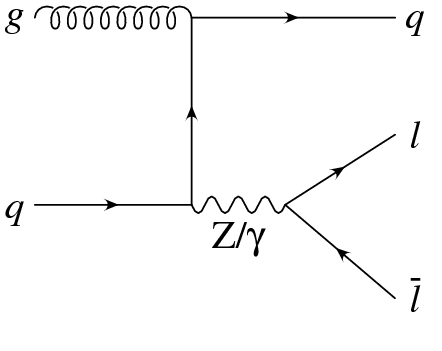
\includegraphics[width=.4\linewidth]{figures/xsection/ZJetsDiagram.png}
    } \\
  \end{center}
  \caption{Feynman diagrams for the most important backgrounds to $\ttbar$ events.  Shown are $Z+Jets$ events (top, left), $W+jets$ events (top, right), QCD events (bottom, left) and Single Top events (bottom, right).}
  \label{img:BackgroundsFeynmanDiagrams}
\end{figure}

To measure the cross-section, the background contributions due to each of the above processes in the lepton+jets channel were determined using a variety of techniques.


\subsection{Dilepton}


\subsection{Combination}




\clearpage
\newpage

\appendix



\section{Statistics}

%Properly using statistical tools ... blah blah blah
Experimental High Energy Physics is uniquely suited for precise, reliable, and accurate statistical analysis.
The detailed knowledge of the underlying physics allow one to create accurate probabilistic models and detailed simulations of measurable physical phenomena.
Large datasets allow these models to be checked, calibrated, and finely tuned to better describe the underlying physics.
Sufficient computational resources are available for massive amounts of simulation to be generated from different models or similar models with various sets of parameters.
Finally, there are a plethora of statistical formulae, tools, and techniques dedicated to the types of measurements performed by High Energy Experimental Physicists.
The above advantages make ATLAS a nearly ideal environment for detailed statistical analysis.

%ATLAS uses a variety of standard statistical techniques for performing measurements.
%The standard set at ATLAS is to use ``frequentist'' techniques, though this is an extremely loaded term.
%Perhaps it is better to say that ATLAS uses ``likelihood'' techniques (a term which is both more specific and leads to less controversy).
%In practice, this means that measurements are made by constructing a likelihood function, which is a real valued function, $L(data | \vec{\alpha})$, whose value is ves the probability of a data point or a set of data points as a function of a number of parameters, $\vec{\alpha}$.

In high energy physics, the process of performing a statistical analysis consists of two separate steps: the modeling of data and the act of measurement using that model.
The first step requires understanding the underlying theory behind a data, the experimental setup that produced the data, and sources of uncertainty or noise that are present in the data.
The second part requires determining what parameters on is interesting in measuring, the types of questions one would like to answer with those measurements, and what mathematical techniques or approximations one is willing to make when making those measurements.


\subsection{Likelihood}
A physical, mathematical, or statistical model of data requires the construction of a likelihood, which is a function that returns the probability of a given dataset under a specified model.
A model is described in terms of its probability density function, or ``pdf'', which returns the probability of generating a measurable value or a set of measurable values, known collectively as the ``data''.
Because it is a function of data that returns a probability, it must be normalized to unity over the space of datasets such that
\begin{equation}
\int pdf(\vec{D}) d\vec{D} = 1
\end{equation}

%A probability density function, or ``pdf'', is a function of a measured value or a set of measured values, known collectively as the ``data'', which evaluates to the probabilty density of a particular model generating that data.
Often, one describes a family of similar pdf's by paramaterizing the density as a function of one or more parameters, which we will refer to as $\theta$.
These parameters may include parameters that one wants to measure, collectively known as the parameter(s) of interested and here referred to as $\mu$, and it may also include additional parameters, known as nuisance parameters and referred to as $\nu$. %writing the density as a function of one or more parameters.
Every pdf in this paramaterized set much individually be normalized over the space of data. 
\begin{equation}
  \int pdf(\vec{x}, \theta) d\vec{x} = 1 \hspace{5mm} \forall \theta %\in \{\theta\}
\end{equation}
%Each individual pdf, , given a family of pdf's that are paramaterized by a real value $\alpha$, each pdf must obey:

A likelihood is a real valued function, $L(data | \vec{\theta})$, whose value is the probability of a point in data space as a function of a number of parameters, $\vec{\theta}$.
While a pdf is required to be normalized over the set of data, a likelihood is not normalized the space of parameters.
%Though they appear similar, likelihoods and pdf's are quite different objects.
%A pdf is required to be strictly normalized over the set of observable data such that:
%This must be true of any given pdf, including every pdf in a paramaterized family of functions.
In contrast, likelihoods are functions of parameters, but aren't normalized over those parameters.
Likelihoods are always associated with data, and they describe how the probability of that data changes as a function of parameters.

%The reason for this difference becomes clear if one interprets a likelihood as a functional of a pdf which maps that pdf onto a dataset to produce a real (positive) number:
One can interpret a likelihood as a functional that maps a probability distribution function, for a given dataset, to a real number:
\begin{equation}
  L: \text{ \{pdf, data\} } \rightarrow [0, 1]% \[0, 1\] \in \mathbb{R}
\end{equation}

%Likelihoods only become useful objects when they are manipulated to produce statistical statements.
%The type of statement that can be made from likelihoods is the source of disagreement between the ``bayesian'' and ``frequentist'' statistical sects.
%We will here take an agnostic position on the philosophical merits of any type of statistical statement, and instead present a common type of statistical statement, used and recommended by the ATLAS collaboration, as well as many other experiments, known as the confidence interval.

%\subsection{Building Likelihoods at ATLAS}

The creation of a likelihood function is often the most important step in an analysis of physical data.
It encapsulates (hopefully) the entirety of one's knowledge about an experiment, including important parameters that one wants to study and theoretical or experimental uncertainties that effect those parameters.
Specific techniques for creating likelihood functions to describe the data measured by the ATLAS experiment are described in section ~\ref{app:histfactory}.

A likelihood serves as the common starting point for statistical techniques (many statistical techniques don't explicitly require a likelihood function, but they often imply the presence of a particular likelihood function).
%frequentist statistical statements (bayesian methods require the use of one or more ``prior'' pdfs in order to make statistical statements).
The majority of statistical measurements performed by the ATLAS collaboration use frequentist techniques (or approximations to strict frequentist techniques).
However, both frequentist and Bayesian techniques require that physical observables be properly modeled and described by a likelihood function.
In the following sections, we will review the concept of hypothesis testing as applied to the ATLAS experiment.
We will then describe two main categories of statistical measurements known as ``confidence intervals'' and ``limit setting.''
%These two quantities are interrelated to one another.


\subsection{Hypothesis Testing}
A typical problem addressed by high energy physics is the comparison of two probability models that describe different underlying physical processes.
At ATLAS, this often means comparing a new physical theory to the Standard Model for the purpose of either claiming discovery or setting limits.
%These two types of tests are applications of a common frequentists procedure to select between potential probabilistic models.
% High Energy Physics at the LHC follows the perscriptions defined by Neyman and Pearson.
In a more general case, one considers two separate physical models, each with their own likelihood functions that describe the same data, which we will refer to as the ``Null'' hypothesis and the ``Alternate'' hypothesis.
At the LHC, the ``Null'' hypothesis is often the Standard Model, and an ``Alternate'' hypothesis may be a new physical process that one is searching for (in the case of the Higgs Boson, the presence of a Higgs is considered an ``Alternate'' hypothesis, even though, in a strict sense, it is necessary for the Standard Model to be mathematically consistent).

The general procedure for performing a hypothesis is to accept one hypothesis or another based on the outcome of an experiment.
Formally, this means considering the full space spanned by all possible outcomes of an experiment and dividing that space into two segments.
If the outcome of the actual experiment performed falls into one part of the space, one chooses to accept the corresponding hypothesis, and if it falls into the other, then one chooses to believe the other hypothesis.
The determination of the boundary between these regions and the probability measure of the two regions is the core challenge of setting up a hypothesis test.

In frequentist hypothesis testing, one treats the two hypotheses being tested in an asymmetric manor.
One first decides upon a threshold for rejecting the background hypothesis, known as the size of the test, or the probability of a Type-I error, or simply as $\alpha$.
This must be chosen by the experimenter and is based on one's willingness to falsely reject the NULL hypothesis (there are commonly accepted values for this number, but any particular choice of value is purely philosophical).
In high energy experimental physics, one often chooses an extremely small value for $\alpha$ to signify that one requires an extremely high degree of confidence to reject commonly accepted physical models, such as the Standard Model.

The choice of $\alpha$ determines the size, or volume, or measure of the space out experimental outcomes that will result in the alternate hypothesis being accepted (and therefore rejecting the null hypothesis).
Given a choice of $\alpha$, one then chooses a region in the space of possible measured data with a total probability measure under the Null hypothesis of size $\alpha$.
We will denote this region as $K_{\alpha}$, emphasizing the fact that the size of the region is determined by the chosen value $\alpha$.

Clearly, there are many such regions (often infinitely many), and the task of choosing an arbitrary volume in data space may seem daunting, as the space of all experimental outcomes can be both conceptually and computationally massive.
Typically, this region is selected by first choosing a ``test statistic,'' which is a mapping of the full space of experimental outcomes to a smaller dimensional space, which is usually the real number line.
With such a function in hand, the task then becomes picking a 1-dimensional region in the range of the Test Statistic such that $P( T(d) \in K_{ \alpha } | NULL) = \alpha$ (typically, this region is determined by picking a cut-off value, $k_{\alpha}$, such that $K_{\alpha} = \{d : T(d) > k_{\alpha} \}$).
Given a region $K_{a}$, the ``power'' of this region is defined to be $1 - \beta$, where $\beta = P(D \in K_{ \alpha } | Alternate)$ and is commonly known as the probability of a Type-II error.
For a chosen size $\alpha$, an ideal test maximizes $\beta$, and better tests have higher values of $\beta$.
In practice, this task boils down to choosing the most powerful test statistic, from which the value of $k_{\alpha}$ and the region in data $K_{\alpha}$ are determined (though, it may take some analytic or computational to determine the value of $k_{\alpha}$).

In the case of comparing two probability models without any parameters (or equivalently, comparing models with fixed parameters), a result known as the Neyman-Pearson lemma states that the most powerful test statistic is the likelihood ratio, defined as the ratio of the likelihoods of data under the two models being compared.
Although this result is powerful, its usefulness is often limited due to the fact that the presence of systematic uncertainties requires one to compare not just two but rather a continuous families of models to each other.
Often, both the null and the alternate hypothesis are parameterized by variables describing a continuum of experimental or theoretical effects.

The presence of systematic uncertainties makes the determination of the region $K_{\alpha}$ more complicated.
One convention is to choose $K_{\alpha}$ such that the supremum of the measure of probability in that region under all possible Null models over the space of parameters is $\alpha$.
In other words, $\alpha = max( \int P(D|\theta) d(D) )$ where the maximum runs over all values of $\theta$.
If the alternate hypothesis is also parameterized, then the power of this test will no longer be well defined, but rather it will depend on the values of the parameters.


\subsection{Confidence Interval}

A common application of frequentist hypothesis testing techniques is the creation of confidence intervals.
A confidence interval is a procedure that produces a set of parameter points that are compatible with measured data, where compatible  in a very specific, well-defined sense.
Each confidence interval is a function of the level of compatibility, here referred to as $\alpha$, which is determined before the interval is created.
An instance confidence interval is a set obtained using measured data, and in a frequentist sense, any given confidence interval either contains the true parameter points or it doesn't.
However, when the procedure for producing a confidence interval is applied over many (hypothetical) realizations of measured data, the true values of the parameters will be contained in the confidence interval at a rate of $\alpha$.

%A confidence inverval is a procedure that maps a likelihood to a set in the space of parameters which describe the pdf domain of the likelihood function.
%This procedure is useful because it has the following property: given many randomly-generated realizations of the dataset described by the likelihood, the set obtained using the confidence interval procedure will contain the true value of a parameter (the one which describes the true pdf) a fixed percentage of the time, where that percentage is known in advance and determines the procedure for obtaining confidence intervals.

%In other words, assuming that we knew the true distribution for a dataset that we're interested in, the following procedure is possible:
The meaning of a confidence interval can be understood as the result of the following abstract procedure:
\begin{itemize}
  \item Assume there exists true pdf, $pdf_{true} = pdf(Data | \vec{\alpha}_{true})$
    %, and assume that a single dataset $D_{0}$ was drawn randomly using that pdf. %which describes how a single realization of a dataset was generated
  \item Create a likelihood function for that pdf over the full space of parameter values: $L(D | \theta)$.
    % where the parameters onsidering the full family of pdf's ${pdf(Data | \theta) \forall \theta \in {\theta}}$, create a likelihood function evaluated on the measured data:
    % \item Create a likelihood function over the space of pdf's and datasets, assuming that the true pdf is contained in the domain of this likelihood function
  \item Choose a confidence level, $\alpha$, which must be a value between 0 and 1.
  \item Using the true pdf, generate many datasets, and for each dataset, create a confidence interval of size $\alpha$. %set in parameter space $S_i$ based on the above procedure.
%  \item For this given confidence level, and using the measured likelihood, create a confidence interval, which is a set $S_i$ in the space of parameters $\vec{\theta}$
    %  \item There exists a specific procedure, based on that chosen confidence level, which produces a set $S_i$ in the space of parameters $\vec{\alpha}$ using our likelihood function, which we denote as the ``confidence interval''.
  \item Given this set of intervals, {$S_i$}, count the fraction which contain $\alpha_{true}$.
  \item As the number of generated datasets approaches infinity, this fraction will approach the confidence level, $\alpha$.
\end{itemize}

Often, confidence intervals are used to convey the magnitude of uncertainty of a parameter given an experiment.
But a confidence interval should not be confused with results that attempt to quantify the probability distribution of a parameter based on an experimental outcome.
A confidence interval is nothing more than a set defined in the above way.
They are useful only as far as one finds such sets useful, and a confidence interval alone can not be used to evaluate the value or utility of a decision based on observed data.
%They are, however, objective means of quantifying data, in the sense that they don't depend on assumptions about parameters other than those that are build into the likelihood function.
%Any other way of arguing for their merit or usefulness is strictly philosophical.
%We will here assume that confidence intervals are a desirable quantity to calculate and will show how they can be obtained for likelihoods that describe data obtained using the ATLAS detector.


\subsection{Neyman Construction}

The actual determination of a confidence interval is often both conceptually and computationally challenging.
A standard way of conceptualizing and constructing confidence intervals is through the use of a ``Neyman Construction.''


%% http://inspirehep.net/record/582577
%% @article{Conrad:2002kn,
%%       author         = ``Conrad, Jan and Botner, O. and Hallgren, A. and Perez de los Heros, Carlos'',
%%       title          = ``{Including systematic uncertainties in confidence
%%                         interval construction for Poisson statistics}'',
%%       journal        = ``Phys.Rev.'',
%%       volume         = ``D67'',
%%       pages          = ``012002'',
%%       doi            = ``10.1103/PhysRevD.67.012002'',
%%       year           = ``2003'',
%%       eprint         = ``hep-ex/0202013'',
%%       archivePrefix  = ``arXiv'',
%%       primaryClass   = ``hep-ex'',
%%       SLACcitation   = ``%%CITATION = HEP-EX/0202013;%%'',
%% }

%% http://inspirehep.net/record/454197
%% @article{Feldman:1997qc,
%%       author         = ``Feldman, Gary J. and Cousins, Robert D.'',
%%       title          = ``{A Unified approach to the classical statistical analysis
%%                         of small signals}'',
%%       journal        = ``Phys.Rev.'',
%%       volume         = ``D57'',
%%       pages          = ``3873-3889'',
%%       doi            = ``10.1103/PhysRevD.57.3873'',
%%       year           = ``1998'',
%%       eprint         = ``physics/9711021'',
%%       archivePrefix  = ``arXiv'',
%%       primaryClass   = ``physics.data-an'',
%%       reportNumber   = ``HUTP-97-A096'',
%%       SLACcitation   = ``%%CITATION = PHYSICS/9711021;%%'',
%% }

%% http://inspirehep.net/record/1081445
%% @article{Rolke:2011na,
%%       author         = ``Rolke, Wolfgang A. and Lopez, Angel M.'',
%%       title          = ``{Estimating a Signal In the Presence of an Unknown Background}'',
%%       journal        = ``Nucl.Instrum.Meth.'',
%%       volume         = ``A685'',
%%       pages          = ``16-21'',
%%       doi            = ``10.1016/j.nima.2012.05.029'',
%%       year           = ``2012'',
%%       eprint         = ``1112.2299'',
%%       archivePrefix  = ``arXiv'',
%%       primaryClass   = ``physics.data-an'',
%%       SLACcitation   = ``%%CITATION = ARXIV:1112.2299;%%'',
%% }

A Neyman Construction is created by considering the set of points in a space consisting of the product of all experimental results and parameter value.
The Neyman construction is performed by creating sets in this space which are used to construct confidence intervals over parameters for all possible observable realizations of an experiment.
% A Neyman Construction is a set of points in the set of parameters and possible measured data, as well as a procedure for using those points to obtain confidence intervals.
The construction is build as follows:
Consider a likelihood function over a space of parameters, $\vec{\theta}$, and over a space of measured data, $\vec{d}$: $L = L(\vec{d} | \vec{\theta} )$.
Pick a value $\alpha$ which represents the size (strength) of the confidence interval to be built.
As is standard in frequentist hypothesis testing, this must be agreed upon in advance.
Then, for each point in parameter space, $\vec{ \theta }$ (recall that there is a 1-to-1 correspondence between likelihood functions and points in parameter space), create an a region over the set of data, ${ \vec{d} }$, known as an ``acceptance region'', which is constructed such that the total probability measure of that region is $\alpha$: ${ \vec{d}_{ \vec{ \theta } } : P( \vec{d} \in \vec{d}_{ \vec{ \theta } } | \vec{ \theta } ) = \alpha }$.
This requires knowing, or at least being able to integrate, the likelihood of data at a fixed point $\vec{\theta}$ (this distribution can be obtained using Monte-Carlo techniques once $\vec{\alpha}$ has been specified).
Of course, there are many (often infinitely many) such regions for a given parameter point.
Therefore, one must decide in advance how an acceptance region is to be constructed given a fixed likelihood function.
Often, this decision is made by creating an ordering rule, which determines the order in which points are used to populate a the region, which is then filled in order until it has total measure $\alpha$.

An acceptance region is constructed for all possible values of $\vec{\theta}$.
The union of every such region (including both the data and the parameter points) is known as the confidence belt: confidence belt = ${ ( \vec{d}, \vec{ \theta }) : ( \vec{d}, \vec{ \theta }) \in \mbox{some acceptance region for some} \vec{ \theta } }$.
%(the name comes from the cases where there is 1 parameter and 1 data value in the likelihood; in more complicated situations, it is better described as a volume or a multidimensional set).
%We do this for all values of theta to define a belt (or, if theta is a vector, we define a volume in parameter space).

Using this set, a confidence region for a given measured data point, $\vec{d}_0$, can be constructed as the union of all points in the confidence belt which include the measured data point: ${ ( \vec{ \theta }, \vec{d}) \in belt : d = d_{0}}$.
Specifically, confidence region for a particular parameter, $\alpha$, is union of all values of alpha in the confidence belt that contain $\vec{d}_0$.

If $\theta_0$ were the true value, all the data would fall in the interval in defined by $\theta_0$ $\alpha$ percent of the time.
In addition, if the data were to fall in the confidence region of $\theta_0$, then the interval of parameter points would include $\theta_0$.
These two imply the statement: $\theta_0$ is in the confidence interval $\iff$ the data falls in the region of the likelihood function L($\theta_0$).
Thus, the coverage of the region is identical to the coverage of the interval, which is $\alpha$.
Therefore, the confidence interval defined by the above construction is guaranteed proper coverage.

In this sense, a confidence interval is the inversion of a hypothesis.
It represents the set of all points in parameter space for which the measured data falls within an acceptance region of size $\alpha$ (given some ordering rule).
For any single parameter in parameter space, the confidence interval is the the union of all points of that parameter that fall in the confidence band (confidence volume) in the full parameter space.

% Kyle:  Said yet another way, to claim a discovery, the confidence interval for the nuisance parameter(s) must be empty (when the construction is made assuming the null hypothesis).

\subsection{Profile Likelihood}

The above procedure is often conceptualized in the case of a 1-dimensional parameter and a single test statistic.
In this case, the confidence belt represents a 1-d region that consists of confidence intervals for every possible value of the test statistic.
However, when one considers a likelihood consisting of numerous nuisance parameters, constructing a single confidence interval for a parameter of interest is no longer well defined.
For each point in the space of nuisance parameters, a different confidence belt is obtained for a single test statistic and a single parameter of interest.

One may desire to construct a confidence interval consisting of the union of all points of that parameter that fall in the confidence band (confidence volume) in the full parameter space.
However, this is usually incredibly difficult to calculate computationally.
Instead, many results at the ATLAS experiment are calculated using an approximation to the above confidence interval using what is known as the ``Profile Likelihood''~\cite{ATL-CONF-2011-034}.
The profile likelihood reduces the dimensionality of the parameter space by eliminating nuisance parameters while maintaining well-understood confidence intervals.

The profile likelihood ratio is defined as
% http://www.slac.stanford.edu/econf/C030908/papers/WEMT004.pdf
\begin{equation}
  \lambda(\sigma_{\ttbar}) = \frac{L(\sigma_{\ttbar}, \hat{\hat{\lum}}, \hat{\hat{\alpha}}_j)}{L(\hat \sigma_{\ttbar}, \hat \lum, \hat \alpha_j)}\,,
\end{equation}

The profile likelihood techniques transforms a full likelihood function (including nuisance parameters) into a function resembling a likelihood of only parameters of interest my minimizing over the the nuisance parameters for each value of the parameter of interest (and including an overall scale of the global minimum of the likelihood function).
This construction is useful because its frequentist properties can be understood generally in the asymptotic regime.
Specifically, the distribution of this ratio under the data approaches a $\chi^2$ distribution as the size of the data increases (in practice, this convergence happens extremely quickly, which underlies the usefulness of the profile likelihood ratio).
Thus, a confidence interval for a parameter of interest can be obtained using the known properties of the $\chi^2$ distribution.
Specifically, a 65\% confidence interval is defined by the region about the global minimum between the points where the negative log likelihood of the profile likelihood ratio equals $-\frac{1}{2}$ of its maximum value.

This can be interpreted as searching for values of the nuisance parameters that make the probability of the data given the full set of parameters as large as possible.
Near the global minimum of the likelihood, this will have the effect of expanding the confidence interval of a parameter of interest since the the worse-case-scenario of the nuisance parameters will be chosen for each value of the parameter of interest, causing the likelihood function to be more flat around the global minimum, and therefore causing confidence intervals to be wider.

%\subsection{Systematic Uncertainties}

\clearpage
\newpage



\chapter{HistFactory}
\label{app:histfactory}

Statistical measurements, including estimates of physical parameters, the setting of confidence intervals, and the setting of upper and lower limits, require the construction of a likelihood function that incorporates one's knowledge of physical theories, experimental properties, and underlying uncertainties.
Moreover, it is a practical requirement that such a likelihood be expressible in software, and that the software be simple, widely applicable, and fast.
To make complicated statistical techniques widely available and to enable the construction of models complicated enough to accurately describe the details of physical theories, particle detectors, and the LHC, physicists built a software library consisting of tools specifically designed for the creation and evaluation of likelihood functions.

HistFactory is a software tool designed to build paramaterized probability density functions and likelihood functions and is specifically designed to use histograms as inputs.
HistFactory is written in c++, is a part of the ROOT framework, and was built using a statistical modeling library called RooFit.
It can be interfaced with as a c++ library or using both XML or python as a front end.
HistFactory produces standard but highly flexible and customizable likelihood functions using minimal input from the end user.
It does this by taking a modular approach to the construction of probability density functions, where terms in a distribution describing different measurements can be built individually or combined to form larger distributions that describe a bigger space of measurements.

HistFactory is designed to allow systematic uncertainties, both theoretical or experimental in source, to be built into a likelihood function and treated consistently throughout a probability density function, properly taking into account correlations between effects that arise from a single source of systematic error.

%% The \HF\ is a tool to build parametrized probability density functions (pdfs) in the \RooFit/\RooStats\ framework based based on simple ROOT histograms organized in an XML file.  The pdf has a restricted form, but it is sufficiently flexible to describe many analyses based on template histograms. The tool takes a modular approach to build complex pdfs from more primative conceptual building blocks.  The resulting PDF is stored in a RooWorkspace which can be saved to and read from a ROOT file.  This document describes the defaults and interface in \ROOT\ 5.32.  Note, \ROOT\ 5.34 provides a C++ and python interface fully interoperable with the XML interface and classes for analytically fitting bin-by-bin statistical uncertainties on the templates.  These developments will be included in a future version of this document.


\section{Preliminaries}

To understand the likelihood functions that are constructed by HistFactory, we will describe a simple example.
Consider a measurement of the rate of a single process that is performed by measuring the distribution a variable over events of an experiment that satisfy a certain, predefined criteria.
This criteria, which is a function of observables, defines the signal region.
Assume that there are two classes of events that are present in the signal region, the signal process whose properties we're interested in measuring, ``S'', and a background process, ``B''.
Denoting the observable we're studying as $x$, we begin by assuming that we know the distribution of this variable under both the signal and background processes individually.
We will refer to these distributions as $f_{\rm S}(x)$ and $f_{\rm B}(x)$, noting that, as probability distribution functions, they each individually integrate to 1.
%Typically in high energy physics, these distributions are modeled as histograms having a finite number of bins.
%If we make this assumption, then we denote $f_{\rm S}$

We will also define a parameter which scales with the expected number of events coming from the signal process in the signal region, which we refer to as the signal strength, or simply $\mu$.
And finally, we introduce a parameter, $B$, that scales with the number of background events.
We will initially assume that this parameter is known and fixed.

%Thus, given a value of the parameter $\mu$, the expected number of events in the $i

%% Let us begin by considering the simple case of a single channel with one signal and one background contribution and no systematics based on the discriminating variable is $x$.  
%% While we will not continue with this notation, let us start with the familiar convention where the number of signal events is denoted as $S$ and the number of background events as $B$.  
%% Similarly, denote the signal and background ``shapes'' as $f_{\rm S}(x)$ and $f_{\rm B}(x)$ and note the these are probability density functions normalized so that $\int dx f(x)=1$.  
%% It is common to introduce a ``signal strength'' parameter $\mu$ such that $\mu=0$ corresponds to the background-only hypothesis  and $\mu=1$ corresponds to the nominal signal+background hypothesis.  
%% This continuous parameter $\mu$ is our parameter of interest.


Thus, given a value of the parameter $\mu$, the distribution of a number of measured values of x is given by:

\begin{eqnarray}
{\cal P}(\{x_1\dots x_n\} | \mu) = \textrm{Pois}(n | \mu S+B) \left[ \prod_{e=1}^n \frac{\mu S f_{\rm S}(x_e) + B f_{\rm B}(x_e)}{\mu S+B}\right ] \; .
\end{eqnarray}

The first term on the right hand side describes the total number of events measured as a Poisson process whose mean is the sum of the expected number of signal and background events.
The remaining of the right side describes the probability of each individual event having the value $x_e$.
In total, this distribution is known as a marked Poisson model.

Often in high energy physics, the distributions $f_{\rm S}(x)$ and $f_{\rm B}(x)$ are described as histograms.
In this case, we denote the signal and background histograms as $\nu_b^{\rm sig}$ and $\nu_b^{\rm bkg}$, where $b$ is the bin index.
In the case of histograms,  marked Poisson process becomes

\begin{eqnarray}
{\cal P}(n_b |\mu) &=&  \textrm{Pois}(n_{\rm tot} | \mu S + B) \left[\, \prod_{b\in\rm bins}\frac{\mu \nu_b^{\rm sig} + \nu_b^{\rm bkg}}{\mu S + B}\right ] \\
&=& \mathcal{N}_{\rm comb} \prod_{b\in\rm bins} \textrm{Pois}(n_b | \mu \nu_{b}^{\rm sig} + \nu_{b}^{\rm bkg}) \; ,
\label{eqn:histpois}
\end{eqnarray}
where $n_b$ is the histogram of the observed data and and $\mathcal{N}_{\rm comb}$ is a constant combinatorial factor that can be neglected for the purpose of statistical analysis.   
Similarly, we denote the histogram of the distribution of $x$ as measured in data by  $n_b$.


%% Now we ask what the probability model is for obtaining $n$ events in the data where the discriminating variable for event $e$ has a value $x_e$; thus the full dataset will be denoted $\{x_1\dots x_n\}$.  First one must include the Poisson probability of obtaining $n$ events when $\mu S + B$ are expected.  Secondly, one must take into account the probability density of obtaining $x_e$ based on the  relative mixture $f_{\rm S}(x)$ and $f_{\rm B}(x)$ for a given value of $\mu$.   Putting those two ingredients together one obtains what statisticians call a ``marked Poisson model'':
%% \begin{eqnarray}
%% {\cal P}(\{x_1\dots x_n\} | \mu)=  \textrm{Pois}(n | \mu S+B) \left[ \prod_{e=1}^n \frac{\mu S f_{\rm S}(x_e) + B f_{\rm B}(x_e)}{\mu S+B}\right ] \; .
%% \end{eqnarray}
%% If one imagines the data as being fixed, then this equation depends on $\mu$ and is called the likelihood function $L(\mu)$.  Simply taking the logarithm of the equation above and remembering that $\textrm{Pois}(n|\nu) = \nu^n e^{-\nu} / n!$ gives us a familiar formula referred to by physicists as an ``extended maximum likelihood fit'' :
%% \begin{eqnarray}\nonumber
%% -\ln L( \mu) &=&  -n \ln(\mu S + B) + (\mu S + B) + \ln n! - \sum_{e=1}^n \ln \left[ \frac{\mu S f_{\rm S}(x_e) + B f_{\rm B}(x_e)}{\mu S+B}\right] \\
%% %&=&\underbrace{ (\mu S + B)}_{\rm extended~term} - \sum_{e=1}^n \ln \left[ \mu S f_{\rm S}(x_e) + B f_{\rm B}(x_e)\right] + \underbrace{\ln n!}_{\rm irrelevant~constant} \; .
%% &=& (\mu S + B) + \ln n!- \sum_{e=1}^n \ln \left[ \mu S f_{\rm S}(x_e) + B f_{\rm B}(x_e)\right]  \; .
%% \end{eqnarray}

%% Since \HF\ is based on histograms, it is natural to think of the binned equivalent of the probability model above.  Denoted the signal and background histograms as $\nu_b^{\rm sig}$ and $\nu_b^{\rm bkg}$, where $b$ is the bin index and the histograms contents correspond to the number of events expected in the data.   We can relate the bin $\nu_b$ and the shape $f(x)$ via
%%  \begin{equation}
%%  \label{eq:shape}
%% %   S \int _{b_e} dx f_S(x_e ) = \nu_{b_e}^{\rm sig}  \hspace{.5in}  \textrm{and}  \hspace{.5in}  f_B(x_e ) = \frac{\nu_{b_e}^{\rm bkg}}{B} \;,
%%     f_S(x_e ) = \frac{\nu_{b_e}^{\rm sig}}{S \Delta_{b_e}}   \hspace{.5in}  \textrm{and}  \hspace{.5in}  f_B(x_e ) = \frac{\nu_{b_e}^{\rm bkg}}{B \Delta_{b_e}} \;,
%% \end{equation}
%% where $b_e$ is the index of the bin containing $x_e$ and $\Delta_{b_e}$ is the width of that same bins.  Note, because the $f(x)$ are normalized to unity we have $S=\sum_b  \nu_{\rm b}^{\rm sig}$ and $B=\sum_b  \nu_{\rm b}^{\rm bkg}$.


%%  Formally one can either write the probability model in terms of a product over Poisson distributions for each bin of the histogram,  or one can also continue to use the unbinned expression above recognizing that the shapes $f(x)$ look like histograms (ie. they are discontinuous at the bin boundaries and constant between them).  Technically, the \HF\ makes a model that looks more like the unbinned expression with a single RooAbsPdf that is ``extended'' with a discontinuous shape in $x$.  Nevertheless, it can be more convenient to express the model in terms of the individual bins.  Then we have
%% \begin{eqnarray}
%% {\cal P}(n_b |\mu)=  \textrm{Pois}(n_{\rm tot} | \mu S + B) \left[\, \prod_{b\in\rm bins}\frac{\mu \nu_b^{\rm sig} + \nu_b^{\rm bkg}}{\mu S + B}\right ] = \mathcal{N}_{\rm comb} \prod_{b\in\rm bins} \textrm{Pois}(n_b | \mu \nu_{b}^{\rm sig} + \nu_{b}^{\rm bkg}) \; ,
%% \end{eqnarray}
%% where $n_b$ is the data histogram and $\mathcal{N}_{\rm comb}$ is a combinatorial factor that can be neglected since it is constant.   Similarly, denote the data histogram is $n_b$.

This is a simple but powerful example of the type of probability distribution function that can be produced by HistFactory.
For a given set of observed data, it can be interpreted as a likelihood function of $\mu$, the parameter of interest.



\section{Generalizations}

HistFactory make it easy to include a number of generalizations of this problem which all one to create flexible and powerful models.
A simple generalization is the inclusion of additional search channels.
The model described above considers a single observable defined in a single signal region.
However, it is common for analyses to define several categories of events defined by different criteria for the purpose of making a measurement.
Each of these categories is known as a search channel, or simply a channel.
Within each channel, one or more discriminating variables are measured.
The total distribution for this variable (or the join distribution if multiple variables are used) is comprised of events coming from many types of physical processes, 
some of which are considered signal and some of which are background.
Each of these underlying physical processes, be it signal or background, is known in ``HistFactory'' as a sample.
A sample may appear in one, several, or all channels considered by an analysis (but only once per channel).
If it appears in more than one channel, it most likely shares a common parameter across channels.
HistFactory is designed to make this sharing of parameters conceptually simple and statistically correct.

A statistical model spanning several search channels can be created by combining likelihoods designed to describe individual search channels.
One can express the joint likelihood function of several channels as the product of the likelihood functions for individual channels (assuming that the probability of an event falling into more than one search channel is, almost surely, zero).
%But if one simultaneously studies a (potentially) different variable in a different signal region (that has no overlap with the original signal region), then one can simply express the joint likelihood function as the prodicut of the individual likelihood functions.
However, when making this product, one should be sure to use a single variable to express common parameters that are meant to be identified across likelihoods.
For example, in the joint likelihood function, one should use a single parameter $\mu$ to describe a signal strength that is coherent across search channels.
One can include any number of channels in this way.
In addition, it is easy to include multiple discriminating variables in each channel by using multidimensional histograms.
Similarly, one can consider any number of background distributions, which simply get added to equation~\ref{eqn:histpois}.

Most importantly, however, is the ability to include parameters to describe systematic uncertainties in additional to the parameter of interest.
HistFactory has developed a number ways to describe the effect of systematic uncertainties, some of which are quite intricate and sophisticated.
For the purpose of explanation, we will here only describe the two most common cases.

The two types of systematic uncertainties modeled by HistFactory that we will describe here are uncertainties that can scale the overall yield of a channel (or several channels coherently), and systematic uncertainties that can effect the shape of binned distributions in a channel (or across several channels coherently).

The first type of uncertainty is modeled by including a parameter per channel and per sample in that channel (if necessary) that scales the overall expected yield from that sample in that channel.
If several samples (either in the same channel or across multiple channels) are effected by the same logical source of systematic uncertainty, each will have a separate parameter that determines the relative size of the change in yield for that each sample individually.
However, because the source of uncertainty is common across those channels, a single, global parameter will control the size, as measured in standard deviations, of the effect, which is then propagated to each sample.
The relative size of the response in each sample to the underlying source of systematic uncertainty is an input provided by the user.
For each source of systematic uncertainty and for each sample effected by the uncertainty, the user provides the relative change in yield (where 1.0 means no change) when the parameter describing the underlying source of systematic uncertainty has a one standard deviation upward fluctuation, and likewise for a downward fluctuation of one standard deviation.
The size of the response for values other than exactly $\pm 1$ sigma are obtained as interpolations between the relative size of the $\pm 1$ sigma response sizes per channel as a function of the parameter describing the underlying source of uncertainty.
In the language of HistFactory, this type of systematic uncertainty is known as an ``OverallSys.''
Typically, a linear interpolation is used, though other schemes are available, and smoother interpolations (which don't have discontinuous derivatives) tend to perform better under gradient descent minimization schemes.

To illustrate, for a channel consisting of only 1 bin, the expected number of events in that channel is given by equation\ref{Eq:alphaInterpolation}.
\begin{eqnarray}\label{Eq:alphaInterpolation}
N^{\text{exp}}_{i, \text{tot}}(\vec{\alpha}) &=& \sum_{\text{background}} N^{\text{exp}}_{i} (1 + \sum_{j} \alpha_{j} \, \Delta N_j  ) \, \\
\Delta N_j &=& \begin{cases} \Delta N^{+}_{j}, & \mbox{if } \alpha_{j} > 0  \\ \Delta N^{-}_{j}, & \mbox{if } \alpha_{j} < 0 \end{cases},
\end{eqnarray}
where $\Delta N^{+}_{j}$ and $\Delta N^{-}_{j}$ are the differences in the expected number of events due to an upward or downward fluctuation
of one standard deviation of the $j^{th}$ nuisance parameter.

This type of systematic uncertainty may be interpreted as a parameter that describes on uncertainty on the overall number of events for either a signal or background signal.
Since it effects an overall expected yield, it is commonly used to describe an uncertainty on an efficiency, including a trigger, identification, or reconstruction efficiency, or an uncertainty on an overall cross-section (as it is commonly used in analysis describe in this thesis).

The second type of uncertainty considered is a natural extension of the ``OverallSys'' category of uncertainties, and is known as a ``HistoSys.''
A HistSys, similar to an OverallSys, is an effect that can vary per sample and per channel (including having no effect) but is controlled by a single, common parameter
that represents the underlying source of systematic uncertainty.
For every sample effected by this source of systematic uncertainty, the user supplies template histograms representing the shape of the distribution of that sample for both the plus 1-sigma and minus 1-sigma values for the global source of systematic uncertainty.
The shape of the discriminating variable for that sample for an arbitrary value of the source of systematic uncertainty comes from a continuous interpolation of those templates.

This type of effect from a systematic uncertainty can be used to describe changes in the shape of distributions that can be attributed to a source of systematic uncertainty.
A common example is the case where a kinematic variable being modeled depends on the energy of jets in the event (such as an invariant mass, or even the number of reconstructed jets).
In this case, an uncertainty on the overall jet energy scale will causes changes in the shape of this discriminating variable.

Both categories of systematic uncertainties described above use a single, global parameter to model the underlying source of that uncertainty.
When building the full likelihood function, constraint terms are added to the likelihood which describe the certainty with which these parameters are known.
Each parameter describing a source of systematic uncertainty is constrained by a Gaussian product in the likelihood.
However, it may be desirable to not include a constraint term on a source of systematic uncertainty.
In HistFactory, a ``NormFactory'' is effectively an ``OverallSys'' that doesn't include a constraint term in the likelihood.
In such a case, the parameter described by the NormFactor is said to ``float'' and is unconstrained in likelihood fits.
This is useful for modeling parameters of interests, and is used throughout the analyses described in this thesis to model the $\ttbar$ cross-section and the various cross-sections of exotic models.

\section{The likelihood function}

HistFactory's more important feature is providing a software representation of the joint likelihood across all channels and including all signals and background considered by an analysis.
This likelihood function describes the distribution of a discriminating variable (or variables) in each channel as a joint, binned distribution (in ROOT, this is supplied by an n-dimensional histogram).
It takes into account the effect of several types of systematic uncertainties, including those described above, as well as parameters of interest.
Moreover, since nearly all analyses made using the ATLAS detector depend on the value of the total integrated luminosity (which has a finite and non-negligible uncertainty),
a parameter describing the systematic uncertainty on the measured integrated luminosity is included by default.
One can turn this effect off for samples that are evaluated in data, meaning their estimates don't depend on the measured value of integrated luminosity (they of course depend on the actual value of integrated luminosity, but not measurements of that value).

The likelihood function created by HistFactory is given by equation~\ref{Eq:HistFactoryLikelihoodTemplate}.

\begin{eqnarray}
\label{Eq:HistFactoryLikelihoodTemplate}
\nonumber
{\cal P}( n_{cb}, a_p \; |\,\phi_p,\alpha_p,\gamma_b)=   \prod_{c\in \textrm{channels}} \; \prod_{b\in \textrm{bins}} \textrm{Pois}(n_{cb}|\nu_{cb}) \cdot G(L_0 | \lambda, \Delta_L) \cdot \prod_{p\in \mathbb{S}+\mathbf{\Gamma}} f_p(a_p|\alpha_p)
\end{eqnarray}

\begin{itemize}
%\item $b_e$ the bin containing $x_e$ (ie. the bin for event $e$)
\item $ \lambda_{cs}$ - luminosity parameter for a given channel and sample.  Within a given channel this parameter is a common luminosity parameter for all the samples that include luminosity uncertainty (i.e.. \texttt{NormalizeByTheory="True"}).  For all the samples with  \texttt{NormalizeByTheory="False"} it is fixed to the nominal luminosity $\lambda_{cs}=L_0$.
\item $\gamma_{cb_e}$ - Bin-by-bin scale factor used for statistical uncertainties, bin-by-bin shape systematics (\SS), and data-driven shape extrapolations (\SF).  For statistical errors, the $\gamma_{csb_e}$ is shared for all the samples in the channel (ie. subscript $s$ can be omitted).  For samples that do not have any bin-by-bin scale factors $\gamma_{csb_e}=1$.
\item $\alpha_p$ - Parameters associated to sources of systematic uncertainty that have constraints
\item $f_p(a_p|\alpha_p)$ - A constraint term describing an auxiliary measurement $a_p$ that constrains a nuisance parameter $\alpha_p$
\item $ \phi_{cs}$ - Product of unconstrained normalization factors for a given sample within a given channel.  These typically include the parameter of interest, eg. the signal cross-section or branching ratio.
 \begin{equation}
 \phi_{cs}= \prod_{p\in\mathbb{N}_c} \phi_p
 \end{equation}
\item $\eta_{cs}(\vec\alpha)$  - The parametrized normalization uncertainties (ie. \OS) for a given sample within a given channel (a factor around 1).
\item $\sigma_{csb_e}$  - The parametrized histogram (ie. the nominal histogram and the \HS) for a given sample within a given channel.
\end{itemize}


\section{Statistical Uncertainties}
Histfactory uses shape templates to model the distributions of signal and background samples.
These templates are typically derived using Monte Carlo simulation or by measuring a distribution
in a control region.
Both of these methods use a number of training events to construct a distribution.
When this number is small, the effect of having finite statistics to construct a
shape template may become important.
To address this issue, HistFactory introduced a sceme that paramaterizes changes in the shapes
of distribution templates 










\clearpage
\newpage

\bibliographystyle{common/atlasnote}
\bibliography{references}

%% Bibliography. I didn't use BibTeX, so you're on your own if you'd like to do so.
%
\begin{thebibliography}{99}\addcontentsline{toc}{chapter}{Bibliography}
\bibitem{JBC91}J.~B.~Conway, \emph{Functions of One Complex
    Variable~I}. Second edition. Springer-Verlag, Graduate
    Texts in Mathematics~\textbf{11}, 1991.
\end{thebibliography}


%% If your thesis has different "Parts", use commands such as the following:
%\part{First Part\label{part:one}}%
%\input{chap2} % further chapters -- change file names to meaningful things...
%\input{chap3}
%\part{Second Part\label{part:two}}%
%\input{chap4}
%\input{chap5}
%\input{chap6}
%%%%% Appendices start %%%%%%%%%%%%%%%%
%% Comment out the following line if your thesis has no appendix
%% Note: If your thesis has more than one appendix, NYU requires a "list of
%% appendices" page before the body of the thesis. I don't provide the tools
%% to create that here, so you're on your own for that one... Sorry.
%\input{app2}
%%%% Input bibliography file %%%%%%%%%%%%%%%

\end{document}
